\documentclass[10pt,conference,compsocconf]{IEEEtran}
\usepackage{tabularx}
\usepackage{subcaption}
\usepackage{hyperref}
\usepackage{graphicx}	% For figure environment
\usepackage{amsfonts}
\usepackage{multirow}
\setlength\parindent{0pt}
\usepackage{amsmath}
\begin{document}
\title{Deep Learning Project 1: Report}

\author{
  Raphael Bonatti\\
  Lena Csomor\\
  Marijn van der Meer\\
  \textit{Department of Computer Science, EPF Lausanne, Switzerland}
}

\maketitle

\section{Introduction}
As a part of the course 'Deep Learning', this group implemented different Machine Learning architectures that compare two digits displayed in an image. We compared the performance improvements are achieved by using specific architectures, different optimisers, weight sharing and auxiliary losses. We started with a baseline model, which is a very basic neural network, and evolved to increasingly sophisticated architectures such as CNNs, RNNs and Siamese Networks. While we tested many architectures that often were very similar to each other, in this report we kept only the ones we deemed interesting and that showed progress in our thought and coding process.

\section{Methods}\label{sec:models-methods}
\subsection{Data Generation}
\label{subsec:data-generation}
As input for the models, the famous MNIST dataset is used. The test and training sets consist of 1000 randomly chosen pairs of images, both 14x14 pixels of grayscale handwritten ciphers. So one sample is of 2x14x14 (Figure~\ref{fig:example-ciphers}). For each pair, the model should predict whether the first digit is lesser or equal to the second. 

\begin{figure}[htbp]
  \centering
  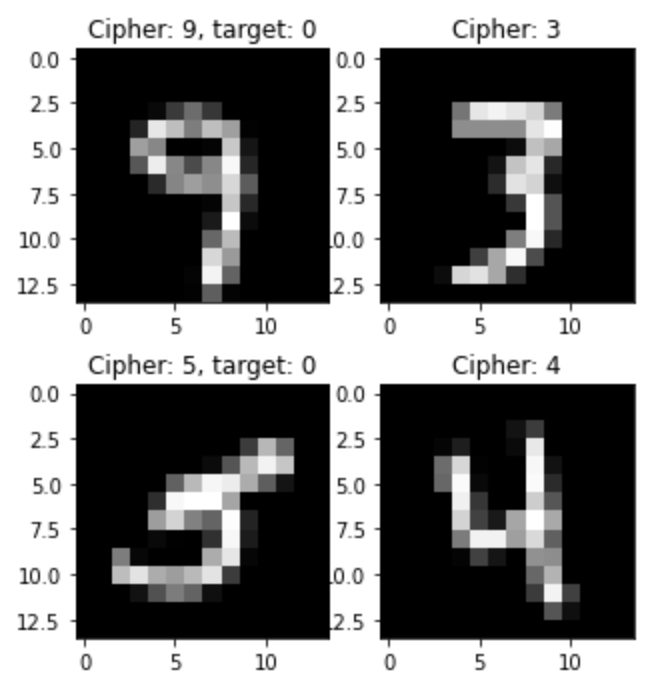
\includegraphics[width=0.5\columnwidth]{doc/project1-report/example_ciphers.png}
  \vspace{-3mm}
  \caption{Examples of data samples used as input to the model. Pairs of grayscale cipher images from MNIST of size 14x14. The target variable of each pair is 1 when the cipher on the first image is smaller or equal to the cipher on the second image.}
  \label{fig:example-ciphers}
\end{figure}


\subsection{Evaluation Metrics}\label{subsec:evaluation-metrics}
As evaluation metrics we chose to use accuracy and F1-score to assess the performance of our model on the test set. We used both measures in case the data set was not well balanced in terms of target values. We also displayed the average loss, which reflects how well the architecture models the data it is given. All performance assessments are aggregated values from at least 10 runs with randomly chosen training and test data sets and, if not indicated otherwise, 50 epochs of training. 

\section{Models}\label{sec:models}
\subsection{Baseline Model}
\label{subsec:baseline-model}
The baseline model is a neural network with only one hidden linear layer. We used softmax as an activation function, the loss is calculated with cross-entropy and the optimizer used is SGD.\\
The network is fully connected, and the two images are flattened into a one-dimensional input tensor. The output consists of 2 logits, where the first describes the probability of the output being zero, while the second describes the output being one.\\
The performance of the baseline can be found in Table~\ref{tab:final-table}. For such a simple model, its performance is already surprisingly good with an average accuracy of 77\% and F1 of 79\%.

\begin{figure}[htbp]
  \centering
  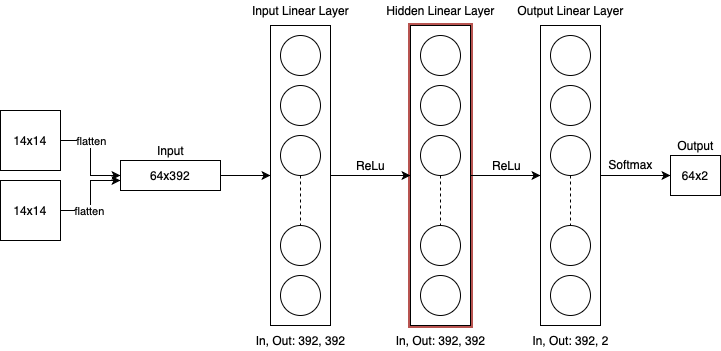
\includegraphics[width=\columnwidth]{doc/project1-report/baseline.png}
  \vspace{-3mm}
  \caption[small]{Visualisation of the baseline model, a fully connected network with one hidden linear layer.}
  \label{fig:baseline}
\end{figure}

%\begin{table}[!t]
%  \centering
%  \begin{tabular}[c]{|l||l|l|}
%    \hline
%    Measure&Average&Standard Deviation\\
%    \hline
%    Accuracy [\%] &76.74&1.3055\\
%    F1 [\%] &78.94&1.4073\\
    %ROC&0.0122&0.0002\\
%    Average Loss&0.0110&0.0009\\
%    \hline
%  \end{tabular}
%  \caption{Performance assessment of the baseline model (Figure~\ref{fig:baseline}). Performance was assessed after 50 epochs by averaging results on the test sets over 10 runs with randomly chosen training and test sets. }
%  \label{tab:performance-baseline}
%\end{table}

\subsection{Siamese Models}\label{subsec:siamese-models}
A Siamese Network contains two sub-networks that are trained in parallel. Each single network uses one half of the input for their computations, such that they output comparable vectors. The two sub-networks can, but do not have to, share weights. In our case, siamese networks are advantageous because our datasamples come in pairs. This way, we can first perform computations on both individual sample of a pair, concatenate the results of both networks and add a final part that will assess whether one cipher is smaller or equal to the other.

We will present different siamese models and assess their performance.\newline

\subsubsection{Linear Siamese Network}\label{subsubsec:siamese-models}
At first, we only focused on simple siamese networks with only linear layers.
The first model is a fully connected siamese network: 
\begin{itemize}
    \item Weight sharing: no 
    \item Activation function: softmax \item Learning rate: $1e-3$
    \item Loss: cross-entropy
    \item Optimizer: SGD
\end{itemize}
The performance roughly matches the baseline model with approximately 75\% accuracy and 77\% F1-score (c.f. Linear Siamese Model 1, Table~\ref{tab:final-table}). 

%\begin{table}[htbp]
%\centering
%\begin{tabular}[c]{|l||l|l|}
%\hline
%Measure&Average&Standard %Deviation\\
%\hline
%Accuracy %(percent)&75.08&1.5664\\
%F1 (percent)&77.6739&1.3844%\\
%AUC&0.8355&0.0141\\
%Average Loss&0.0086&0.0005\\
%\hline
%\end{tabular}
%\caption{Performance assessment of Linear Siamese Model 1. Performance was assessed after 50 epochs by averaging results on the test sets over 10 runs with randomly chosen training and test sets. }
%\label{tab:performance-siamese1}
%\end{%table}

This model was extended by adding shared weights (Figure~\ref{fig:siamese2}). As can be seen in Figure~\ref{fig:siamese2}, the two outputs of the siamese parts are concatenated, flattened and entered into a last linear layer before getting the final logits. With a 75\% accuracy and 78\% F1-score (c.f. Linear Siamese Model 2, Table~\ref{tab:final-table}), adding weight sharing does not improve the performance of this model significantly nor exceed the baseline, so we concentrated on more sophisticated, deeper models.

\begin{figure}[htbp]
  \centering
  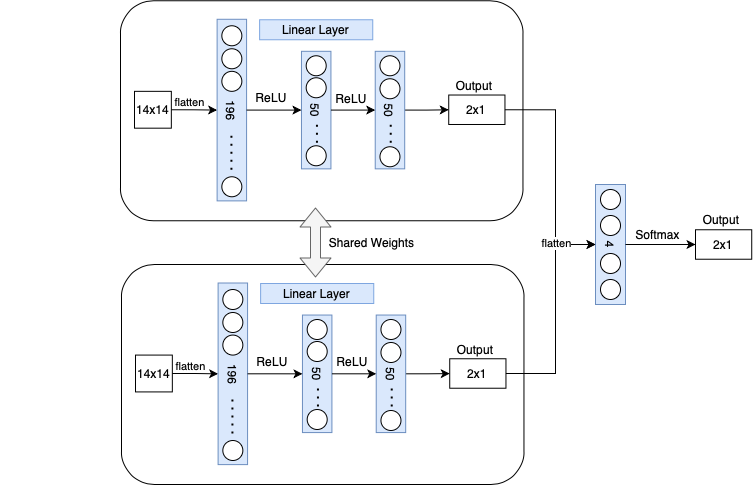
\includegraphics[width=\columnwidth]{doc/project1-report/linear_siamese.png}
  \vspace{-3mm}
  \caption{Visualisation of Linear Siamese Model with shared weights.}
  \label{fig:siamese2}
\end{figure}

%\begin{table}[htbp]
%\centering
%\begin{tabular}[c]{|l||l|l|}
%\hline
%Measure&Average&Standard Deviation\\
%\hline
%Accuracy (percent)&75.58&1.5747\\
%F1 (percent)&78.1692&1.4938%\\
%AUC&0.8387&0.0179\\
%Average Loss&0.0084&0.0007\\
%\hline
%\end{tabular}
%\caption{Performance assessment of Linear Siamese Model with shared weights. Performance was assessed after 50 epochs by averaging results on the test sets over 10 runs with randomly chosen training and test sets. }
%\label{tab:performance-siamese2}
%\end{table}

\subsubsection{Convolutional Siamese Network}\label{subsubsec:convolutional-networks}
We replaced linear with convolutional layers which can reduce the total number of units in a network, and thus also reduced the number of parameters. Convolutional units also consider the context of their neighbourhood, which is very important in image processing task such as ours. \newline
\subsubsection*{Model 1}
We started with a siamese network with 3 convolutional layers that is fully connected at the end:
\begin{itemize}
    \item Weight sharing: no 
    \item Activation function: softmax \item Learning rate: $1e-3$
    \item Loss: cross-entropy
    \item Optimizer: SGD
\end{itemize}

Architecturally, it is the same as Model 2 presented below, but without weight sharing. Even though this model is more complex than the baseline, the performance still does not exceed the baseline with 75\% accuracy and 76\% F1-score (c.f. Siamese CNN 1, Table~\ref{tab:final-table}). \newline
%\begin{table}[htbp]
%\centering
%\begin{tabular}[c]{|l||l|l|}
%\hline
%Measure&Average&Standard Deviation\\
%\hline
%Accuracy (percent)&75.38&1.6067\\
%F1 (percent)&76.7598&2.2532\\
%AUC&0.8416&0.0103\\
%Average Loss&0.0088&0.0004\\
%\hline
%\end{tabular}
%\caption{Performance assessment of Convolutional Siamese Model 1 without shared weights. Performance was assessed after 50 epochs by averaging results on the test sets over 10 runs with randomly chosen training and test sets. }
%\label{tab:performance-siamese3}
%\end{table}

\subsubsection*{Model 2}
In a next step, we added shared weights to the CNN siamese network \textit{Model 1} (Figure~\ref{fig:siamese4}).
\begin{itemize}
    \item Weight sharing: yes 
    \item Activation function: softmax
    \item Loss: cross-entropy
    \item Learning rate: $1e-3$
    \item Optimizer: SGD
\end{itemize}
This improves performance slightly with 77\% accuracy and 79\% F1-score (c.f. Siamese CNN 2, Table~\ref{tab:final-table}), with an increase of around one percent compared to the baseline. \newline

\begin{figure}[!t]
  \centering
  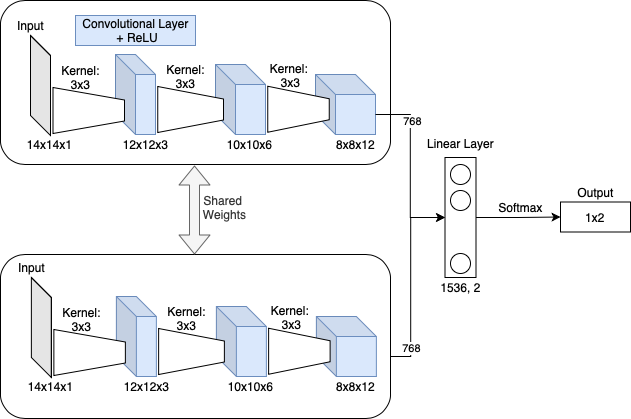
\includegraphics[width=\columnwidth]{doc/project1-report/siamese4.png}
  \vspace{-3mm}
  \caption{Visualisation of Convolutional Siamese Model 1 with shared weights.}
  \label{fig:siamese4}
\end{figure}

%\begin{table}[htbp]
%\centering
%\begin{tabular}[c]{|l||l|l|}
%\hline
%Measure&Average&Standard Deviation\\
%\hline
%Accuracy (percent)&77.67&1.5441\\
%F1 (percent)&79.7918&1.1749\\
%AUC&0.8573&0.0152\\
%Average Loss&0.0083&0.0007\\
%\hline
%\end{tabular}
%\caption{Performance assessment of Convolutional Siamese Model 2 with shared weights. Performance was assessed after 50 epochs by averaging results on the test sets over 10 runs with randomly chosen training and test sets.}
%\label{tab:performance-siamese4}
%\end{table}

\subsubsection*{Model 3}
Not satisfied with the results so far, we built a more complex model and integrated auxiliary losses (Figure~\ref{fig:siamese5}). This model consists of a siamese network with convolutional layers and 
\begin{itemize}
    \item Shared weights: yes
    \item Loss: cross-entropy
    \item Optimiser: Adam
    \item Learning rate: $1e-3$
    \item Activation function: softmax
    \item Other features: max pooling and dropout
\end{itemize}
This model uses auxiliary losses, meaning each part of the siamese network first predicts the cipher on the image (inside of rectangle in Figure~\ref{fig:siamese5}). The logits of these sub-parts are then concatenated and flattened and used as input to a linear layer that predicts the final binary logits. The auxiliary loss is used to evaluate the cipher predictions of the sub-parts of the model. For training, the total loss that is evaluated is calculated as the a weighted sum of all losses: 
\begin{equation}\label{eq:weighted-loss}
    \text{l} = w_1*\text{aux-loss}_1+w_2*\text{aux-loss}_2+w_3*\text{final-loss}
\end{equation}
Where $\text{aux-loss}_1$ and $\text{aux-loss}_2$ evaluate the cipher prediction and $\text{final-loss}$ the final binary output prediction. \textit{Model 3} uses $w = [0.8, 0.8, 1]$ as weights for the weighted loss. The performance of this model is much better and even higher than the baseline with 81\% accuracy and 82\% F1-score (c.f. Siamese CNN 3, Table~\ref{tab:final-table}). We note also that the accuracy of the cipher predictions is already high with 79\% accuracy. 

\begin{figure}[htbp]
  \centering
  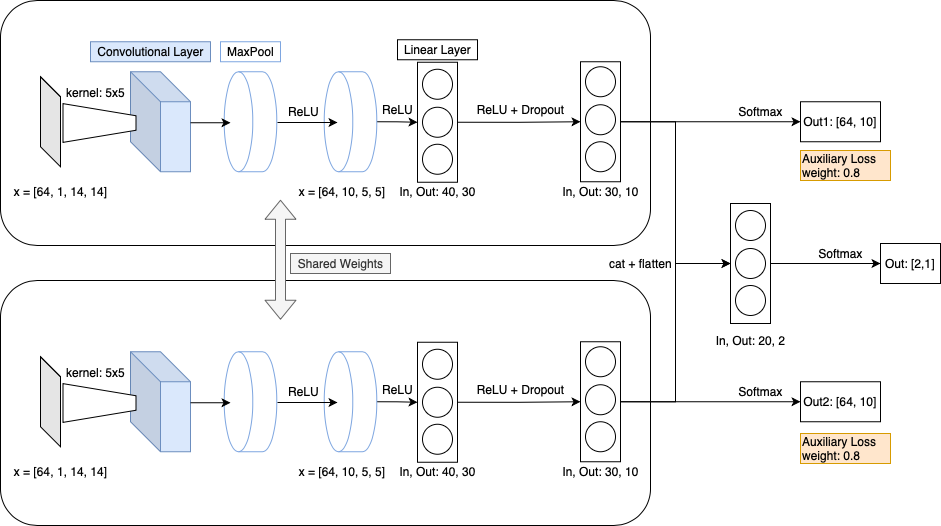
\includegraphics[width=\columnwidth]{doc/project1-report/cnnsiamese.png}
  \vspace{-3mm}
  \caption{Visualisation of CNN Siamese Model with auxiliary losses.}
  \label{fig:siamese5}
\end{figure}

%\begin{table}[htbp]
%\centering
%\begin{tabular}[c]{|l||l|l|}
%\hline
%Measure&Average&Standard Deviation\\
%\hline
%%Accuracy (percent)&81.03&2.9799\\
%F1 (percent)&82.56&3.1201\\
%Accuracy Ciphers (percent)&79.01&4.8458\\
%Average Loss&0.0243&0.0031\\
%\hline
%\end{tabular}
%\caption{Performance assessment of CNN Siamese Model with auxiliary and shared weights. Performance was assessed after 100 epochs by averaging results on the test sets over 10 runs with randomly chosen training and test sets.}
%\label{tab:conv_basic}
%\end{table}

\subsection{RNN Siamese Network}
In a next sequence of experiments, we tried siamese networks with a recurrent neural sub-network instead of a CNN. Recurrent neural networks have an internal state memory and are often used for tasks such as handwriting recognition for example, which we thought could match our task well. More specifically, we used Elman RNN's which consists of three layers and a set of context units that form the internal memory. We initialised the hidden weights to 0 and use tanh as activation function.The siamese network consists of two Elman RNN which are fully connected at the end. Their outputs are flattened, concatenated and put through another linear layer to give the final result (Figure~\ref{fig:siamese6}). The model also relies on auxiliary losses.
\begin{itemize}
    \item Weight sharing: yes 
    \item Activation function: tanh in RNN and softmax for final logits
    \item Loss: cross-entropy
    \item Learning rate: $1e-3$
    \item Optimiser: Adam
    \item Weights for total loss: $w = [0.8, 0.8, 1]$ (Eq.\ref{eq:weighted-loss})
\end{itemize}

The performance is below the baseline at this point with 71\% accuracy and 74\% F1-score (Siamese RNN 1, able~\ref{tab:final-table}). We see that compared to the previous CNN, the cipher accuracy is lower with  51\%. Unlike to the CNN architectures that are run for 100 epochs, the Siamese RNN were run only for 50 epochs because after 50 it started to highly overfit to the training set. 

%\begin{table}[htbp]
%\centering
%\begin{tabular}[c]{|l||l|l|}
%\hline
%Measure&Average&Standard Deviation\\
%\hline
%Accuracy (percent)&71.4&2.0244\\
%F1 (percent)&74.17278&1.2061\\
%Accuracy Ciphers (percent)&50.8545&0.55\\
%Average Loss&0.0432&0.0013\\
%\hline
%\end{tabular}
%\caption{Performance Assessment RNN Siamese Model. Performance was assessed after 50 epochs by averaging results on the test sets over 10 runs with randomly chosen training and test sets.}
%\label{tab:image-rnn}
%\end{table}

%\begin{table}[htbp]
%\centering
%\begin{tabular}[c]{|l||l|l|}
%\hline
%Measure&Average&Standard Deviation\\
%\hline
%Accuracy (percent)&71.42&2.0670\\
%F1 (percent)&74.23&2.4225\\
%Accuracy Ciphers (percent)&58.25&3.5251\\
%Average Loss&0.0501&0.0020\\
%\hline
%\end{tabular}
%\caption{Performance Assessment RNN Siamese Model with Longer Linear Model. Performance was assessed after 50 epochs by averaging results on the test sets over 10 runs with randomly chosen training and test sets.}\label{tab:longer-rnn}
%\end{table}

We also experimented with the same architecture, but with a longer linear model at the end and tried training for a longer period of time. This did not improve the performance in any way  with 71\% accuracy, 74\% F1-score and 58\% accuracy on ciphers (Siamese RNN 2, Table~\ref{tab:final-table}). We suspect that a reason why performance was not improved with a longer linear model is because the final output is mainly determined by how well the network recognises the individual ciphers, which is done in the RNN and not the linear layer.

\subsection{Best Model}
As our best model we returned to CNN siamese networks. However, this time we decided to go a step further and make it even deeper to improve Siamese CNN 3 (Figure~\ref{fig:best-performance}). 
This model consists of 6 convolutional layers, each doubling the number of channels. In the middle, we also added batch normalisation to make the architecture more stable and dropout to reduce overfitting. We also use ReLU between layers and keep using dropout between the last three convolutional layers. This model also uses auxiliary losses.
\begin{itemize}
    \item Weight sharing: yes 
    \item Activation function: softmax
    \item Loss: cross-entropy
    \item Learning rate: $1e-3$
    \item Optimiser: Adam
    \item Weights for total loss: $w = [0.8, 0.8, 1]$ (Eq.\ref{eq:weighted-loss})
\end{itemize}

After training this architecture for 100 epochs, we finally reached an overall accuracy of over 85\% and F1-score of 87\%, while the accuracy in cipher prediction is 92\% (Table~\ref{tab:final-table}). The evolution of evaluation metrics and losses during over the epochs can be seen in Figure~\ref{fig:best-metrics}.

%\begin{table}[htbp]
%\centering
%\begin{tabular}[c]{|l||l|l|}
%\hline
%Measure&Average&Standard Deviation\\
%\hline
%Accuracy (percent)&85.77&0.7655\\
%F1 (percent)&86.98&0.5811\\
%Accuracy Ciphers (percent)&91.92&0.5618\\
%Average Loss&0.0184&0.0019\\
%\hline
%\end{tabular}
%\caption{Performance Assessment Deep Siamese CNN. Performance was assessed after 100 epochs by averaging results on the test sets over 10 runs with randomly chosen training and test sets.}
%\label{tab:siam-conv-net2}
%\end{table}





\section{Summary}
In conclusion, the best model we found for this task is a deep siamese network CNN network. Our optimal model uses both auxiliary losses to predict the ciphers on the image pairs and a final loss to produce a binary output. It also uses shared weights between the siamese modules. This model provided the best final accuracy (85\%) and cipher  prediction (92\%). Compared to RNN or linear siamese structures, CNN models took longer to train, but they reached better performances than the other architectures without overfitting. In further work to try to improve the accuracy, we could try going even deeper as this strategy seemed to work best. We should also explore other optimisers and data pre-processing or augmentation techniques.  

%\bibliographystyle{IEEEtran}
%\bibliography{literature}
\newpage
\onecolumn 
\section{Appendix}
\begin{figure}[htbp]
  \centering
  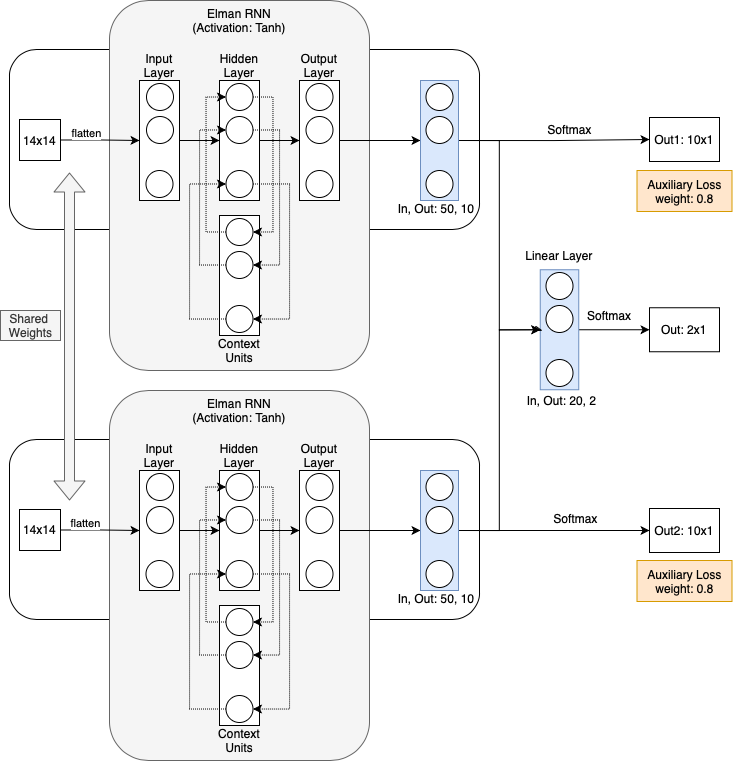
\includegraphics[width=0.5\textwidth]{doc/project1-report/siamese_rnn.png}
  \vspace{-3mm}
  \caption{Visualisation of RNN Siamese Model.}
  \label{fig:siamese6}
\end{figure}

\begin{figure}[htbp]
  \centering
  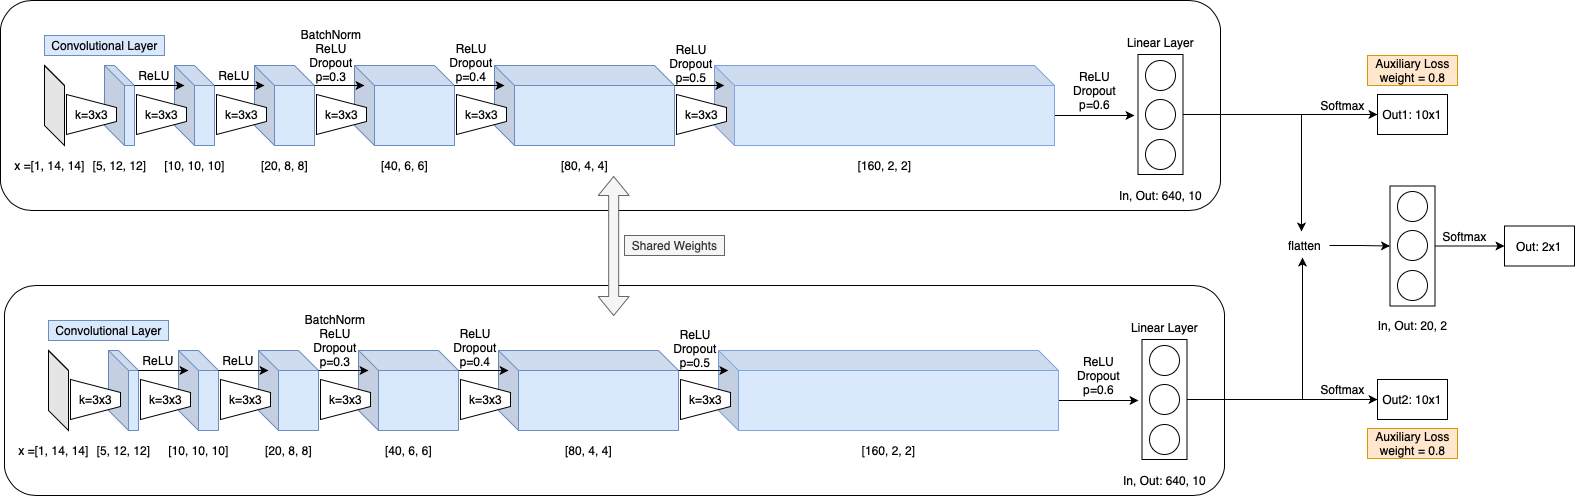
\includegraphics[scale=0.35]{doc/project1-report/bestmodel.png}
  \vspace{-3mm}
  \caption{Visualisation of Deep Siamese CNN Model}
  \label{fig:best-performance}
\end{figure}

\begin{figure}[htp]
        \centering
        \begin{subfigure}[b]{0.45\columnwidth}
            \centering 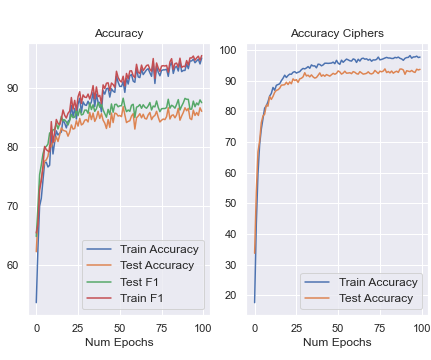
\includegraphics[width=\textwidth]{doc/project1-report/best_model_vis_acc.png}
            \caption[]%
            {\small Evaluation metrics of Deep Siamese CNN over 100 epochs. On the left metrics on the final binary prediction and on the right accuracy on cipher prediction. }   
     \label{fig:best-loss}
        \end{subfigure}
                \hfill 
        \begin{subfigure}[b]{0.45\columnwidth}
            \centering 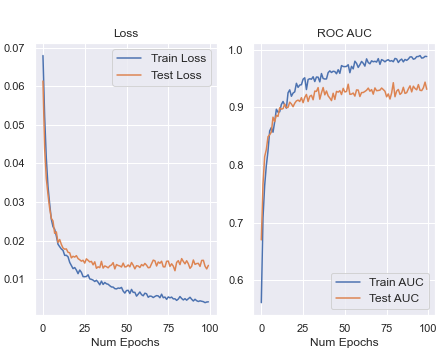
\includegraphics[width=\textwidth]{doc/project1-report/best_model_vis_loss.png}
            \caption[]%
            {\small On the left, taining (blue) and test loss (orange) for 100 epochs. On the right, AUC metric on training (blue) and test (orange) sets for 100 epochs. }     \label{fig:best-accuracy}
        \end{subfigure}
        \caption[]
        {Loss and evaluation metrics for training and testing of Deep Siamese CNN model (Figure~\ref{fig:best-performance}).}
        \label{fig:best-metrics}
    \end{figure}


% Please add the following required packages to your document preamble:
% \usepackage{multirow}
\begin{table}[]
\centering
\begin{tabular}{|llcccc|}
\hline
\textbf{Model}                                            & \textbf{Measure}            & \multicolumn{1}{l}{\textbf{Accuracy}} & \multicolumn{1}{l}{\textbf{F1}} & \multicolumn{1}{l}{\textbf{Cipher Accuracy}} & \multicolumn{1}{l|}{\textbf{Loss}} \\ \hline
\multirow{2}{*}{\textbf{Baseline}}               & Mean            & 76.74                        & 78.94                  & -                                   & 0.0110                    \\
                                                 & Std & 1.3055                       & 1.4073                 & -                                   & 0.0009                    \\ \hline
\multirow{2}{*}{\textbf{Linear Siamese Model 1}} & Mean            & 75.08                        & 77.67                  & -                                   & 0.0086                    \\
                                                 & Std & 1.5664                       & 1.3844                 & -                                   & 0.0005                    \\ \hline
\multirow{2}{*}{\textbf{Linear Siamese Model 2}} & Mean            & 75.58                        & 78.16                  & -                                   & 0.0084                    \\
                                                 & Std & 1.5747                       & 1.4938                 & -                                   & 0.0007                    \\ \hline
\multirow{2}{*}{\textbf{Siamese CNN 1}}          & Mean            & 75.38                        & 76.75                  & -                                   & 0.0088                    \\
                                                 & Std & 1.6067                       & 2.2532                 & -                                   & 0.0004                    \\ \hline
\multirow{2}{*}{\textbf{Siamese CNN 2}}          & Mean            & 77.67                        & 79.79                  & -                                   & 0.0083                    \\
                                                 & Std & 1.5441                       & 1.1749                 & -                                   & 0.0007                    \\ \hline
\multirow{2}{*}{\textbf{Siamese CNN 3}}          & Mean            & 81.03                        & 82.56                  & 79.01                               & 0.0243                    \\
                                                 & Std & 2.9799                       & 3.1201                 & 4.8458                              & 0.0031                    \\ \hline
\multirow{2}{*}{\textbf{Siamese RNN 1}}          & Mean            & 71.40                        & 74.17                  & 50.85                               & 0.0432                    \\
                                                 & Std & 2.0244                       & 1.2061                 & 0.5553                              & 0.0013                    \\ \hline
\multirow{2}{*}{\textbf{Siamese RNN 2}}          & Mean            & 71.42                        & 74.23                  & 58.25                               & 0.0501                    \\
                                                 & Std & 2.0670                       & 2.4225                 & 3.5251                              & 0.0020                    \\ \hline
\multirow{2}{*}{\textbf{Best Model}}             & Mean            & 85.77                        & 86.98                  & 91.92                               & 0.0184                    \\
                                                 & Std & 0.7655                       & 0.5811                 & 0.5618                              & 0.0019                    \\ \hline
\end{tabular}
\caption{Performance of all models explored in this report. Performance was assessed after 50 epochs for all except CCN models (Siamese CNN 1,2,3 and best model) which were run for 100 epochs for by averaging results on the test sets over 10 runs with randomly chosen training and test sets.}
\label{tab:final-table}
\end{table}



\end{document}
